\appendix

\section{Analysis of the dataset with air speed measurements at three heights}\label{sec:analysis-of-the-dataset-with-air-speed-measurements-at-three-heights}

In this section, we analyzed the dataset with air speed measurements at three heights.
Only a limited subset of papers in the \ac{db2} had air speed measurements at three heights with \ac{v}~$\geq$~\qty{0.2}{\m\per\s}.
A summary of the papers is provided in Table~\ref{tab:three_heights_papers}.
The table also shows the number of measurements for each paper and how much (percentage) each study contributed to the dataset.
\begin{table}[htb!]
    \centering
    \begin{tabular}{lrr}
\toprule
Publication & Count & \% Total \\
\midrule
Cena, K., and de Dear, R. J. (1999) & 827 & 27 \\
de Dear, R.J. and Fountain, M.E. (1994) & 704 & 23 \\
Zhang, Y., Chen, H., Meng, Q. (2013) & 465 & 15 \\
Zhang, Y. et al. (2010) & 416 & 14 \\
Schiller (Brager), G. (1990) & 304 & 10 \\
Donnini, G. et al. (1996) & 192 & 6 \\
Tartarini, F., Cooper, P., Fleming, R. (2018) & 113 & 4 \\
Benton, C. C. and Brager, G. S. (1994) & 30 & 1 \\
\bottomrule
\end{tabular}

    \caption{F1-score for the \ac{pmv} and \ac{pmv-ce} models for different subsets of data.}
    \label{tab:three_heights_papers}
\end{table}
The paper by Cena et al.\ (1999), de Dear et al. (1994), and Zhang et al.\ (2013 and 2010) contributed the most to the dataset.
These \num{3063} entries where used to compare the \ac{pmv} and \ac{pmv-ce} models using the same methodology as in Section~\ref{sec:results}.
The air speed distribution at the three heights for each paper is shown in Figure~\ref{fig:boxenplot_wind_speed_three_heights}.
\begin{figure}[htb!]
    \centering
    
\includegraphics[width=\textwidth]{figures/boxenplot_wind_speed_three_heights}
    \caption{Wind speeds distribution at three heights.}
    \label{fig:boxenplot_wind_speed_three_heights}
\end{figure}
The distribution of air speed at the three heights varies between the papers, hence, it is difficult to make generalizations.
However, it should be noted that in most of the studies the air speed measured at the chest height was a good representation of the air speed at the other two heights.
This assumption is not valid for Brenton et al.\ (1994) however this study contributed only \qty{1}{\percent} of the dataset.
The adjustment of \ac{v} based on the \ac{met} significantly increased the base value of the air speed measured by all the studies.
With the value of \ac{v} being \var{delta_v_mean} higher than the average of the other wind speeds combined.
The discussion on weather this increase is justified is beyond the scope of this paper since both Standards require the user to adjust the air speed based on the \ac{met} value.

In this section we are not showing the F1-score for the \ac{pmv} and \ac{pmv-ce} models for the different subsets of data since we have already presented the results in Table~\ref{tab:f1}.
We would like to remind the reader that the F1-macro score for \ac{pmv-ce}~=~\num{.16} was lower than the \ac{pmv}~=~\num{.17} for this subset of data, i.e, \ac{v}~$\geq$~\qty{0.2}{\m\per\s} and \ac{v} measured at three heights.
As previously discussed this is an unexpected result since the \ac{pmv-ce} should be significantly more accurate than the \ac{pmv} model for this subset of data to justify its use.
In this section we are not showing the accuracy of the \ac{pmv} and \ac{pmv-ce} model as a function of the \ac{tsv} since we have a very limited number of measurements for this subset of data moreover this analysis has several limitations as previously discussed.

We, however, plotted the \ac{pmv} and \ac{pmv-ce} values against the \ac{tsv} values and we plotted the \ac{lowess} curves to visualize the prevailing data trend.
The results are shown in Figure~\ref{fig:bubble_models_vs_tsv_three_heights}.
\begin{figure*}[htb!]
    \centering
    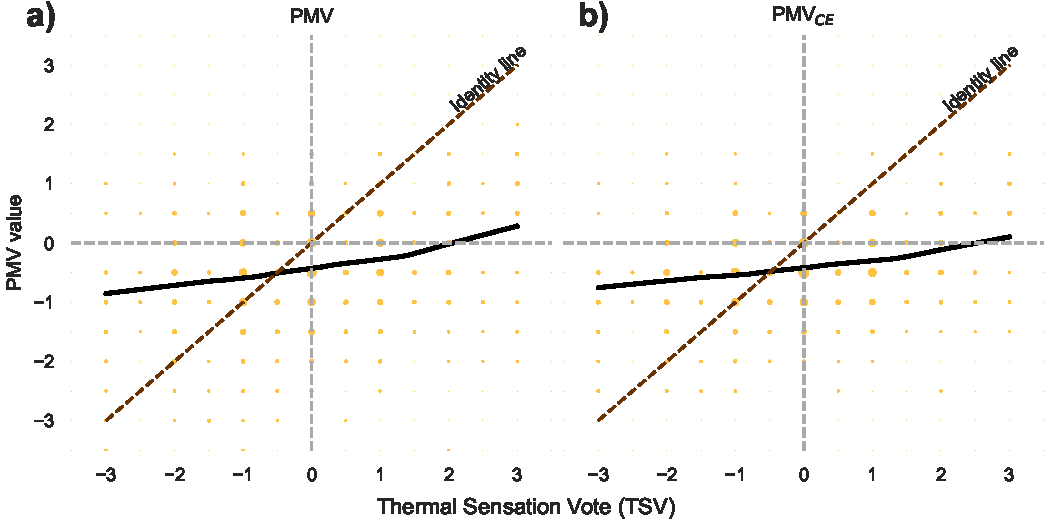
\includegraphics[width=\textwidth]{figures/bubble_models_vs_tsv_three_heights}
    \caption{The \ac{lowess} curve shows the relationship between the raw \ac{pmv} and \ac{tsv} data for the dataset with \ac{v}~$\geq$~\qty{0.2}{\m\per\s} and measured at three heights.
    Raw data were then binned and a bubble chart (circle area is proportional to the number of votes in that bin) was superimposed over the regression curve to aid the visualization of a large dataset.
    The brown dashed line represents the identity line where the slope is 1 and the intercept is 0.
    Comparison between the \ac{pmv} and \ac{pmv-ce} models for the dataset with air speed measured at three heights.}
    \label{fig:bubble_models_vs_tsv_three_heights}
\end{figure*}
The results show that the \ac{pmv} model is more accurate than the \ac{pmv-ce} model.
The intercept of the \ac{pmv} model is \num{-.31} while the intercept of the \ac{pmv-ce} model is \num{-.41}.
Moreover, the \ac{pmv-ce} \ac{lowess} curve is only marginally higher than \num{0} despite participants reporting a \ac{tsv} of \num{3}.

Finally, we are showing calculated the overall bias of the \ac{pmv} and \ac{pmv-ce} models.
The results are shown in Figure~\ref{fig:hist_discrepancies_three_heights}.
\begin{figure}[htb!]
    \centering
    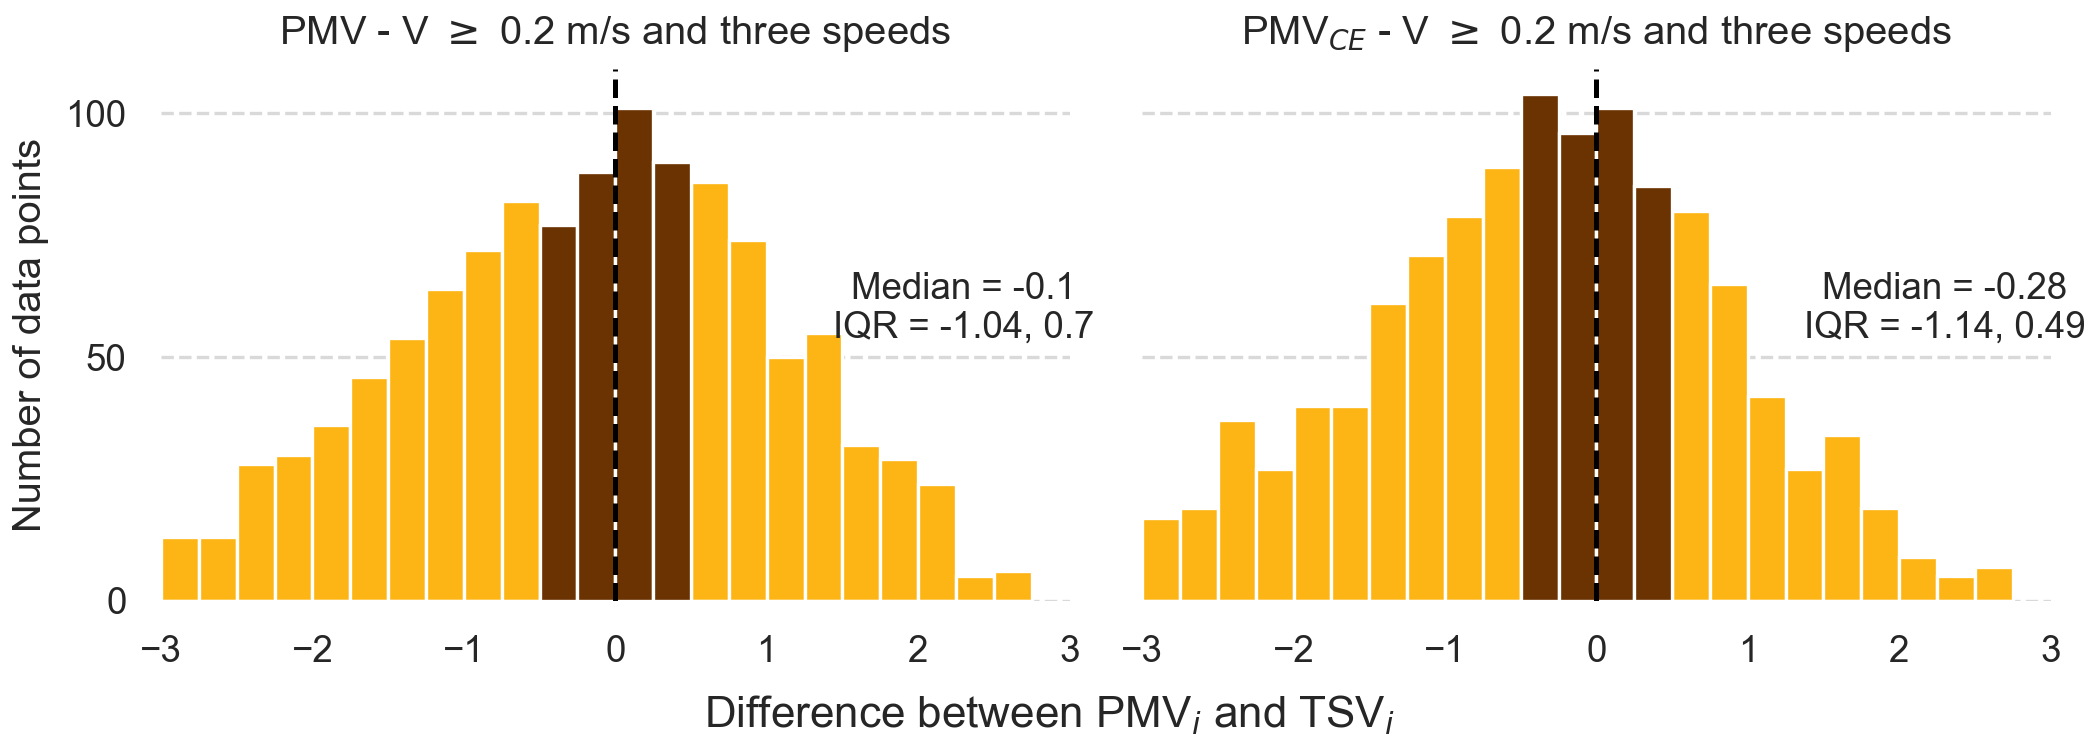
\includegraphics[width=\textwidth]{figures/hist_discrepancies_three_heights}
    \caption{Bias of the \ac{pmv} and \ac{pmv-ce} models for the dataset with air speed measured at three heights.}
    \label{fig:hist_discrepancies_three_heights}
\end{figure}
The \ac{pmv} model has a bias of \num{-.28} while the \ac{pmv-ce} model has a bias of \num{-.38}.
The inter-quartile range for the \ac{pmv} model is more centered around \num{0} than the \ac{pmv-ce} model.
These results allow us to conclude that the \ac{pmv} model is more accurate than the \ac{pmv-ce} model for the dataset with air speed measured at three heights.
Consequently, we recommend using the \ac{pmv} model instead of the \ac{pmv-ce}.

%\section{Comparison between the PMV formulations with the \ac{pmvg}}\label{sec:comparison-between-the-pmv-formulations-with-the-two-node-model}
%We compared how the results of the \ac{pmv} and \ac{pmv-ce} perform against the results of the \ac{pmvg}.
%% SS provide more information why this was done
%% Stefano Schiavon: Please provide more details of how these inputs were generated, within which ranges, etc.
%Figure~\ref{fig:pmv_two_node_comparison} was generated by calculating the three \ac{pmv} values using the same combination of \num{10000} randomly generated sets inputs.
%The \ac{pmv} and \ac{pmv-ce} were then plotted on the y-axis while the \ac{pmvg} value was on the x-axis.
%The Figure also shows the \ac{lowess} curves that are used to visualize the prevailing data trend.
%% Stefano Schiavon: Beside the visualization, can you discuss here also the quantitative results to support the conclusion?
%The results of the \ac{pmv} model had a higher agreement than those obtained with the \ac{pmv-ce} model for \ac{pmvg} $\geq$ \qty{0.5}{\m\per\s}.
%% Stefano Schiavon: This is unclear and cannot be deduced from the figure, from where does it come from? How can a PMV model be described by an air speed?
%These results show the \ac{pmv-ce} is less similar to the \ac{pmvg} model than the \ac{pmv}, despite using it in the backend to calculate the cooling effect.
%This is also an unexpected result and we will discuss why this may be in the following paragraph.
%% SS When a figure report how well a variable is predicted, for example x-measured vs x-predicted, the graph must be a square, otherwise it is visually skewed. 1) I suggest to use the words instead of numbers for PMV 2) We should be consistent with the PMV naming we used (do not use ASHRAE and ISO here) 3) why both models are far from Gagge for PMV<0, both model in general produce a cooler feeling than PMVgagge, we should explain why if we keep this paper.
%
%\begin{figure*}[htb!]
%    \centering
%    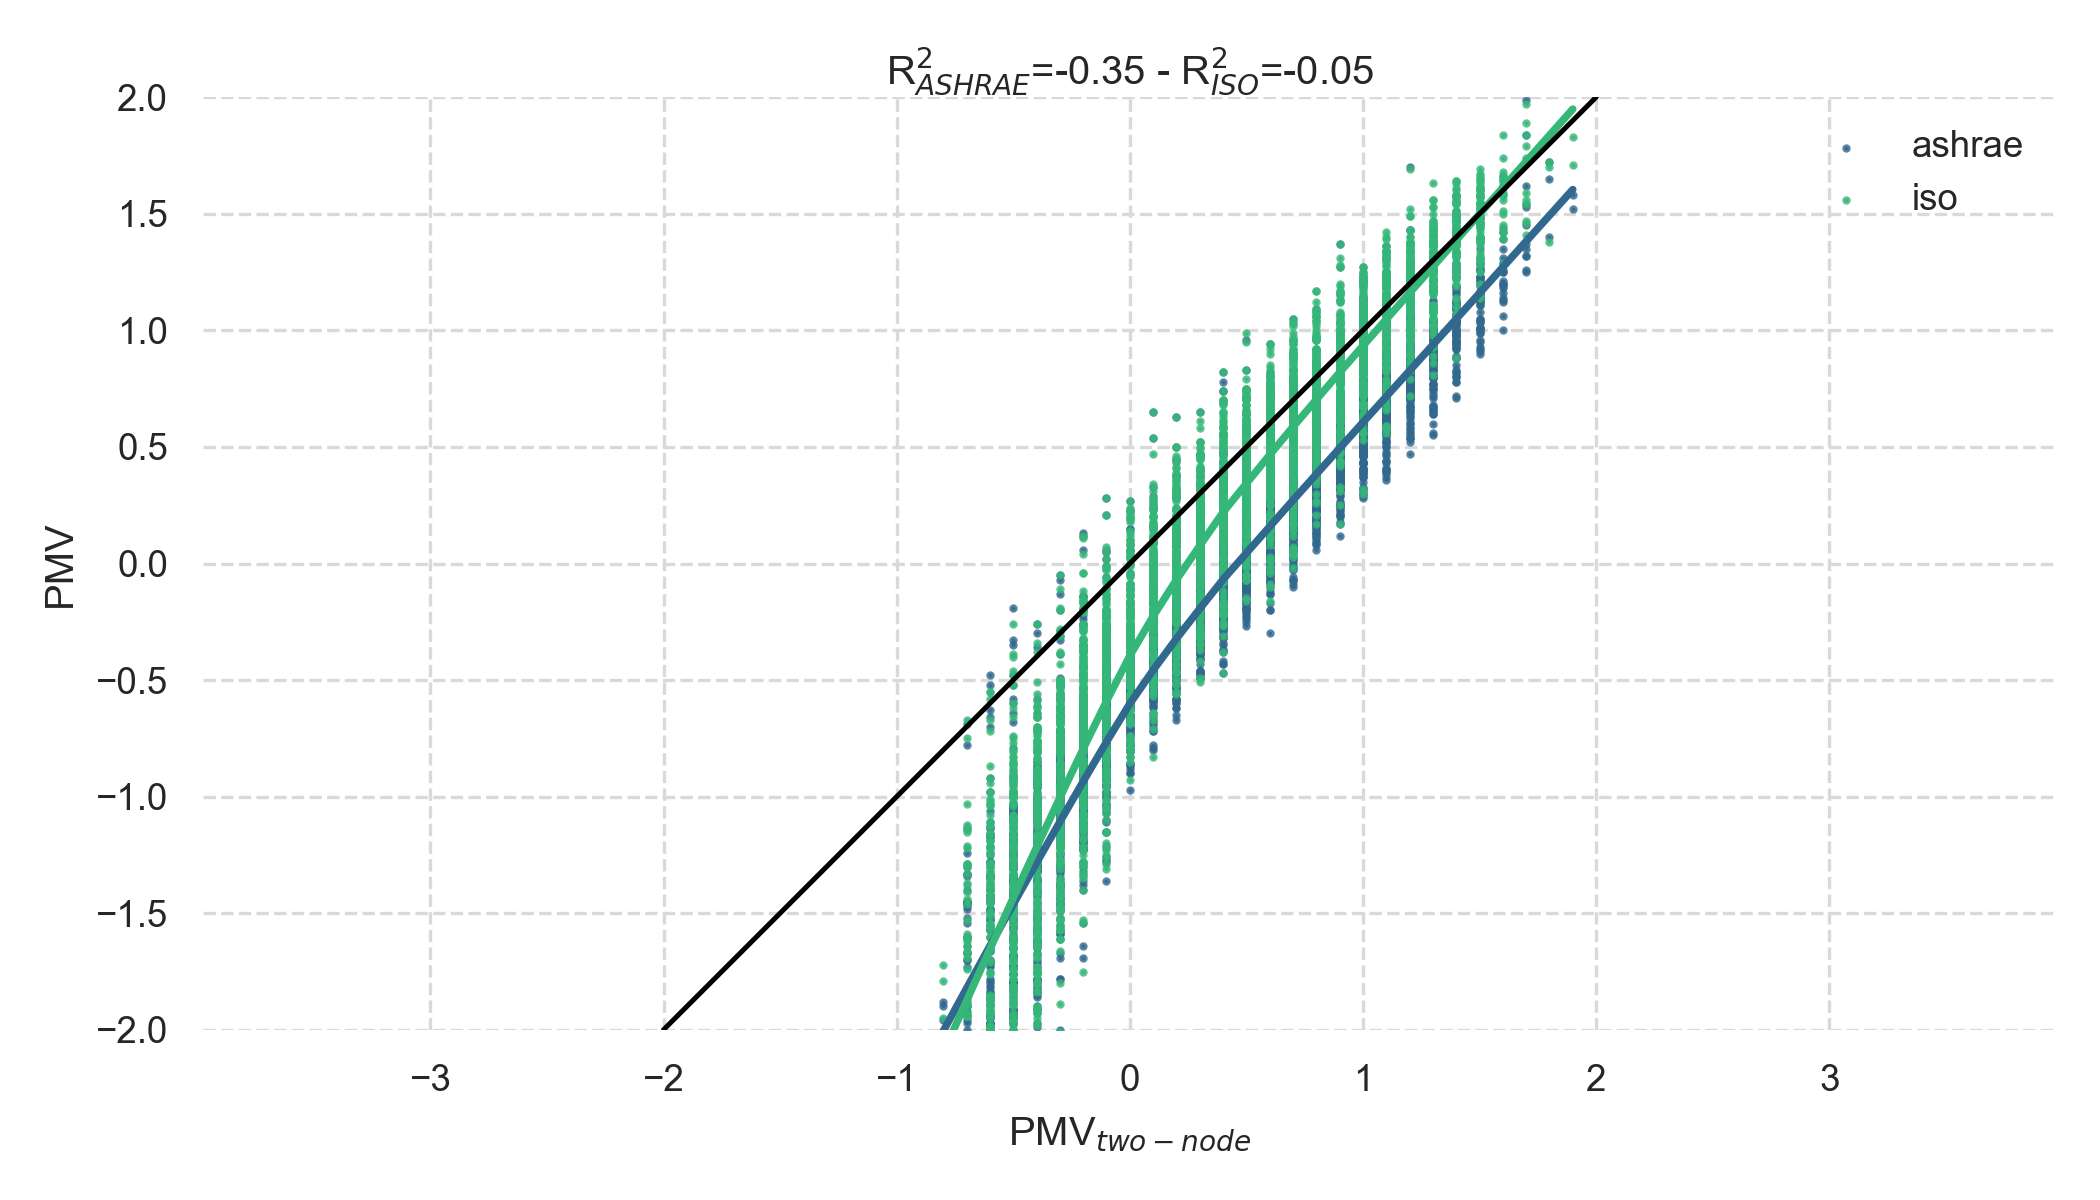
\includegraphics[width=\textwidth]{figures/pmv_two_node_comparison}
%    \caption{}
%    \label{fig:pmv_two_node_comparison}
%\end{figure*}